% ŠABLONA PRO PSANÍ ZÁVĚREČNÉ STUDIJNÍ PRÁCE
%%%%%%%%%%%%%%%%%%%%%%%%%%%%%%%%%%%%%%%%%%%%
% Autor: Jakub Dokulil (kubadokulil99@gmail.com)
% Tato šablona byla vytvořena tak, aby pomocí ní mohli v systému LaTeX soutěžící sázet své práce a zároveň odpovídala požadavkům na formátování vyplývajícím z wordové šablony umístěné na webu soc.cz.
%
\documentclass[12pt, a4paper,
oneside,      %% -- odkomentujte, pokud chcete svou práci mít pouze jednostrannou, mezera pro hřbet pak automaticky bude pouze na levé straně
        %% -- pro oboustranné práce, mezera pro hřbet následně střídá strany.
openright
]{report}

%% Nutné balíčky a nastavení
%%%%%%%%%%%%%%%%%%%%%%%%%%%%

%% Proměnné
\newcommand\obor{INFORMAČNÍ TECHNOLOGIE} %% -- napiš číslo a název tvého oboru
\newcommand\kodOboru{18-20-M/01} %% -- napiš číslo a název tvého oboru
\newcommand\zamereni{se zaměřením na počítačové sítě a programování} %% -- napiš číslo a název tvého oboru
\newcommand\skola{Střední škola průmyslová a umělecká, Opava} %% vyplň název školy
\newcommand\trida{IT4} %% vyplň jméno svého konzultanta
\newcommand\jmenoAutora{Mai Anh Perinová}  %% vyplň své jméno
\newcommand\skolniRok{2023/24} %% vyplň rok
\newcommand\datumOdevzdani{1. 1. 2024} %% vyplň rok
\newcommand\nazevPrace{HaruDolore} %% vyplň název své práce

% předefinování příkazu chapter
\let\oldchapter\chapter
\renewcommand{\chapter}{
	\clearpage %Zajišťuje že nová kapitola začne na nové stránce
	\pagestyle{plain} %Nastavuje styl stránky, který chcete používat
	\oldchapter	
}

\title{\nazevPrace} %% -- Název tvé práce
\author{\jmenoAutora} %% -- tvé jméno
\date{\datumOdevzdani} %% -- rok, kdy píšeš SOČku

\usepackage[top=2.5cm, bottom=2.5cm, left=3.5cm, right=1.5cm]{geometry} %% nastaví okraje, left -- vnitřní okraj, right -- vnější okraj

\usepackage[czech]{babel} %% balík babel pro sazbu v češtině
\usepackage[utf8]{inputenc} %% balíky pro kódování textu
\usepackage[T1]{fontenc}
\usepackage{cmap} %% balíček zajišťující, že vytvořené PDF bude prohledávatelné a kopírovatelné

\usepackage{graphicx} %% balík pro vkládání obrázků

\usepackage{subcaption} %% balíček pro vkládání podobrázků

\usepackage{hyperref} %% balíček, který v PDF vytváří odkazy

\linespread{1.25} %% řádkování
\setlength{\parskip}{0.5em} %% odsazení mezi odstavci


\usepackage[pagestyles]{titlesec} %% balíček pro úpravu stylu kapitol a sekcí
\titleformat{\chapter}[block]{\scshape\bfseries\LARGE}{\thechapter}{10pt}{\vspace{0pt}}[\vspace{-22pt}]
\titleformat{\section}[block]{\scshape\bfseries\Large}{\thesection}{10pt}{\vspace{0pt}}
\titleformat{\subsection}[block]{\bfseries\large}{\thesubsection}{10pt}{\vspace{0pt}}


\usepackage{tocloft} % Balíček umožní přizpůsobit vzhled tabulky obsahu
\setlength{\cftbeforechapskip}{0pt}  % Menší rozestup pro kapitoly
\setlength{\cftbeforesecskip}{0pt}   % Menší rozestup pro sekce

\setcounter{secnumdepth}{2}
\setcounter{tocdepth}{2}
\usepackage{fancyhdr}
\pagestyle{fancy}
\renewcommand{\headrulewidth}{0.025pt}

\usepackage{booktabs}

\usepackage{url}

%% Balíčky co se můžou hodit :) 
%%%%%%%%%%%%%%%%%%%%%%%%%%%%%%%

\usepackage{pdfpages} %% Balíček umožňující vkládat stránky z PDF souborů, 

\usepackage{upgreek} %% Balíček pro sazbu stojatých řeckých písmen, třeba u jednotky mikrometr. Například stojaté mí: \upmu, stojaté pí: \uppi

\usepackage{amsmath}    %% Balíčky amsmath a amsfonts 
\usepackage{amsfonts}   %% pro sazbu matematických symbolů
\usepackage{esint}     %% pro sazbu různých integrálů (např \oiint)
\usepackage{mathrsfs}
\usepackage{helvet} % Helvet font
\usepackage{mathptmx} % Times New Roman
\usepackage{Oswald} % Oswald font


%% makra pro sazbu matematiky
\newcommand{\dif}{\mathrm{d}} %% makro pro sazbu diferenciálu, místo toho
%% abych musel psát '\mathrm{d}' mi stačí napsat '\dif' což je mnohem 
%% kratší a mohu si tak usnadnit práci

\usepackage{listings}
\usepackage{xcolor}

\renewcommand{\lstlistingname}{Kód}% Listing -> Algorithm
\renewcommand{\lstlistlistingname}{Seznam programových kódů}% List of Listings -> List of Algorithms

%% Definice 
\lstdefinelanguage{JavaScript}{
	morekeywords=[1]{break, continue, delete, else, for, function, if, in,
		new, return, this, typeof, var, void, while, with},
	% Literals, primitive types, and reference types.
	morekeywords=[2]{false, null, true, boolean, number, undefined,
		Array, Boolean, Date, Math, Number, String, Object},
	% Built-ins.
	morekeywords=[3]{eval, parseInt, parseFloat, escape, unescape},
	sensitive,
	morecomment=[s]{/*}{*/},
	morecomment=[l]//,
	morecomment=[s]{/**}{*/}, % JavaDoc style comments
	morestring=[b]',
	morestring=[b]"
}[keywords, comments, strings]


\lstdefinelanguage[ECMAScript2015]{JavaScript}[]{JavaScript}{
	morekeywords=[1]{await, async, case, catch, class, const, default, do,
		enum, export, extends, finally, from, implements, import, instanceof,
		let, static, super, switch, throw, try},
	morestring=[b]` % Interpolation strings.
}

\lstalias[]{ES6}[ECMAScript2015]{JavaScript}

% Nastavení barev
% Requires package: color.
\definecolor{mediumgray}{rgb}{0.3, 0.4, 0.4}
\definecolor{mediumblue}{rgb}{0.0, 0.0, 0.8}
\definecolor{forestgreen}{rgb}{0.13, 0.55, 0.13}
\definecolor{darkviolet}{rgb}{0.58, 0.0, 0.83}
\definecolor{royalblue}{rgb}{0.25, 0.41, 0.88}
\definecolor{crimson}{rgb}{0.86, 0.8, 0.24}

\lstdefinestyle{JSES6Base}{
	backgroundcolor=\color{white},
	basicstyle=\ttfamily,
	breakatwhitespace=false,
	breaklines=false,
	captionpos=b,
	columns=fullflexible,
	commentstyle=\color{mediumgray}\upshape,
	emph={},
	emphstyle=\color{crimson},
	extendedchars=true,  % requires inputenc
	fontadjust=true,
	frame=single,
	identifierstyle=\color{black},
	keepspaces=true,
	keywordstyle=\color{mediumblue},
	keywordstyle={[2]\color{darkviolet}},
	keywordstyle={[3]\color{royalblue}},
 literate=%
{á}{{\'a}}1 {č}{{\v{c}}}1 {ď}{{\v{d}}}1 {é}{{\'e}}1 {ě}{{\v{e}}}1
{í}{{\'i}}1 {ň}{{\v{n}}}1 {ó}{{\'o}}1 {ř}{{\v{r}}}1 {š}{{\v{s}}}1
{ť}{{\v{t}}}1 {ú}{{\'u}}1 {ů}{{\r{u}}}1 {ý}{{\'y}}1 {ž}{{\v{z}}}1,		
	numbers=left,
	numbersep=5pt,
	numberstyle=\tiny\color{black},
	rulecolor=\color{black},
	showlines=true,
	showspaces=false,
	showstringspaces=false,
	showtabs=false,
	stringstyle=\color{forestgreen},
	tabsize=2,
	title=\lstname,
	upquote=true  % requires textcomp
}

\lstdefinestyle{JavaScript}{
	language=JavaScript,
	style=JSES6Base,
}
\lstdefinestyle{ES6}{
	language=ES6,
	style=JSES6Base
}


%% Bordel pro práci - můžeš smáznout :) 
%%%%%%%%%%%%%%%%%%%

\usepackage{lipsum} %% balíček který píše lipsum (nesmyslný text, který se používá pro kontrolu typografie)

%% Začátek dokumentu
%%%%%%%%%%%%%%%%%%%%
\begin{document}
	
	\pagestyle{empty}
	\pagenumbering{Roman}
	
	\cleardoublepage

%% Titulní stránka s informacemi
%%%%%%%%%%%%%%%%%%%%%%%%%%%%%%%%%%%%%%%%
	
	{\fontfamily{phv}\selectfont
		%% Logo školy
		\begin{figure}[h]
			\centering
			
\includegraphics[width=0.6\linewidth]{image/logo-skoly.png} 
		\end{figure}
		
		
		%% Hlavička práce a její název (viz proměnná \nazev prace)
		%% \sffamily %%% bezpatkové písmo - sans serif
		{\bfseries %%% písmo na stránce je tučně
			\begin{center}
				\vspace{0.025 \textheight}
				\LARGE{ZÁVĚREČNÁ STUDIJNÍ PRÁCE}\\
				\large{dokumentace}\\
				\vspace{0.075 \textheight}
				\LARGE {\nazevPrace}\\
			\end{center}  
		}%%%
		
		\begin{figure}[h]
			\centering
			
\includegraphics[width=0.8\linewidth]{image/homepage.png} 
		\end{figure}
		
		\vspace{0.02 \textheight}
		\begin{table}[h!]
			\begin{tabular}{ll}
				\textbf{Autor:} & \jmenoAutora\\ 
				\textbf{Obor:} & \kodOboru { } \obor\\
				\textbf{} & \zamereni\\
				\textbf{Třída:} & \trida\\
				\textbf{Školní rok:} & \skolniRok\\
			\end{tabular}
			
		\end{table}		
	}
	
\clearpage %% Zalomení stránky
	
%% Stránka obsahující poděkování a prohlášení
%%%%%%%%%%%%%%%%%%%%%%%%%%%%%%%%%%%%%%%%%%%%%%%%%%%%%%%%
	
	\vspace*{0.7\textheight} %% Vertikální mezeru je možné upravit

%% Prohlášení - povinné
%%%%%%%%%%%%%%%%%%%%%%%%%%%%
	\noindent{\large{\bfseries{Prohlášení}\\}}  %% uprav si koncovky podle toho na jaký rod se cítíš, vypadá to pak lépe :) 
	\noindent{Prohlašuji, že jsem závěrečnou práci vypracoval samostatně a uvedl veškeré použité 
		informační zdroje.\\}
	\noindent{Souhlasím, aby tato studijní práce byla použita k výukovým a prezentačním účelům na Střední průmyslové a umělecké škole v Opavě, Praskova 399/8.}
	\vfill
	\noindent{V Opavě \datumOdevzdani\\}
	\noindent
	\begin{minipage}{\linewidth}
		\hspace{9.5cm} 
		\begin{tabular}{@{}p{6cm}@{}}
			\dotfill \\
			Podpis autora
		\end{tabular}
	\end{minipage}
	
	\clearpage %% Zalomení stránky

%% Stránka obsahující abstrakt (anotaci)
%%%%%%%%%%%%%%%%%%%%%%%%%%%%%%%%%%%%%%%%%%%%%%%%%%%%%%%%	

%% Abstrakt v češtině
%%%%%%%%%%%%%%%%%%%%%%%%%%%%
	\noindent{\Large{\bfseries{Abstrakt}\\}}
	Výsledkem projektu je funkční webová aplikace pro ukládání souborů k určité maturitní otázce. Aplikace umožňuje přihlášení uživatele přes Email, Google, GitHub a Microsoft. Stránka obsahuje maturitní otázky, které jsou rozděleny do určitých kategorií a jsou přehledně zobrazeny. Uživatel si vybírá otázku ke které pak přidá výukový soubor. Soubory se ukládají ke každé otázce zvlášť a jsou k dispozici ke stažení pro přihlášeného uživatele. Každý uživatel vidí pouze své uložené soubory. Při nahrávání výukového matetirálu musí uživatel soubor zařadit do kategorie, která se pak zobrazuje jako štítek vedle nahraného souboru. Vedle štítku se pak nachází tlačítko, které umožňuje smazání souboru.
	\\
	
	\vspace{18pt}
	
	\noindent{\large{\bfseries{Klíčová slova}}}
	
	\noindent webová stránka, databáze, uživatelské účty, soubory \dots 
	
	\vspace{20pt}
	
	%% Abstrakt v angličtině
	%%%%%%%%%%%%%%%%%%%%%%%%%%%%
	
	\noindent{\Large{\bfseries{Abstract}\\}}
	The result of the project is a functional web application for storing files for a specific graduation question. The application allows user login via Email, Google, GitHub and Microsoft. The site contains graduation questions that are divided into specific categories and are clearly displayed. The user chooses a question to which they then add a educational file. The files are stored for each question separately and are available for download to the logged-in user. Each user can only see their own saved files. When uploading a educational material, the user must categorize the file, which is then displayed as a label next to the uploaded file. Next to the label, there is a button allowing the user to delete the file.
	\\
	
	\vspace{18pt}
	
	\noindent{\large{\bfseries{Keywords}}}
	
	\noindent website, database, user accounts, files \dots
	
	\vspace{18pt}
	
	\clearpage %% Zalomení stránky

%% Stránka s generovaným obsahem
%%%%%%%%%%%%%%%%%%%%%%%%%%%%%%%%%%%%%%%	
	
	\tableofcontents %% Vygeneruje tabulku s obsahem

	\pagenumbering{arabic} %% Nastavení způsobu číslování stránek (alternativy roman | Roman)
	\setcounter{page}{1} %% Nastavení počitadla stránek

%% Stránka s úvodem - povinná část
%%%%%%%%%%%%%%%%%%%%%%%%%%%%%%%%%%%%%%%		
	\chapter*{Úvod}
%Tento příkaz vytvoří novou kapitolu s názvem "Úvod" ve vašem dokumentu.
%Hvězdička * u příkazu \chapter* znamená, že tato kapitola nebude mít číslo. Ve výsledném dokumentu se tedy objeví jako "Úvod" bez předcházejícího čísla kapitoly, které se obvykle zobrazuje u číslovaných kapitol.
%Tento příkaz také znamená, že kapitola se automaticky neobjeví v obsahu, protože LaTeX standardně zahrnuje do obsahu pouze číslované kapitoly.
	\addcontentsline{toc}{chapter}{Úvod}
%Tento příkaz ručně přidává záznam do obsahu.
%První parametr toc označuje, že přidáváme záznam do Table of Contents (obsahu).
%Druhý parametr chapter specifikuje úroveň záznamu. V tomto případě říkáme, že přidávaný záznam má být považován za kapitolu.
%Třetí parametr Úvod je text, který se objeví v obsahu. V tomto případě bude v obsahu zobrazen název "Úvod".	
Úvod

%Tipy k psaní úvodu
%Je povinný, nadpis neměňte, rozsah - max. 1 strana. 
%Tato část práce obsahuje: 
%* náhled do řešené problematiky, zdůvodnění volby problematiky, 
%* předem definované cíle práce, 
%* motivaci pro další čtení textu včetně stručného uvedení obsahu následujících kapitol 


\chapter{Backend}
\label{sec:backend}

\section{Next.js 13}
Next.js je framework pro React určený k tvorbě plně vybavených webových aplikací. K vytváření uživatelských rozhraní se používají React komponenty a Next.js se využívá pro další funkce a optimalizace.

Využité výhody z Next.js:
\begin{itemize}
	\item Vykreslování na straně serveru (SSR)
	\item Optimalizace SEO
	\item Optimalizace obrázků
	\item Optimalizace fontů
	\item funkce generateStaticParams
	\item <Link> komponent
	\item Server komponenty
\end{itemize}

\subsection{Optimalizace obrázků}
	Komponent Next.js Image rozšiřuje HTML element <img> o funkce pro automatickou optimalizaci obrázků:
\begin{itemize}
	\item Optimalizace velikosti: Automatické zobrazování obrázků ve správné velikosti pro každé zařízení pomocí moderních formátů, jako jsou WebP a AVIF.
	\item Vizuální stabilita: Automatická prevence posunu rozvržení při načítání obrázků.
	\item Rychlejší načítání stránek: Obrázky se načítají pouze ve chvíli, kdy vstoupí do zobrazovacího prostoru pomocí nativního líného načítání prohlížeče, s volitelnými zástupnými znaky rozmazání.
	\item Flexibilita prostředků:  Možnost změny velikosti obrázků na vyžádání, a to i pro obrázky uložené na vzdálených serverech.
\end{itemize}

\subsection{Optimalizace fontů}
Automaticky optimalizuje font (včetně vlastních fontů) a odstraňuje externí síťové požadavky, čímž zlepšuje soukromí a výkon.

'next/font' obsahuje vestavěný automatický selfhosting pro jakýkoli soubor fontů. Webové fonty se optimálně načítají bez jakéhokoli posunu v rozložení díky podkladovému CSS.

\vspace{10pt}

\begin{lstlisting}[style=JavaScript, title={Kód}, caption={Ukázka layout.js}]
	import { Albert_Sans } from "next/font/google";
	
	const albert = Albert_Sans({
		subsets: ["latin"],
		weight: ["200", "500", "700", "800", "900"],
	});
\end{lstlisting}	

\subsection{Funkce generateStaticParams}
Funkce generateStaticParams je zde využita ke generování slugů pro subject a question na základě dat získaných z databáze. Využívá objekt klienta k provedení dotazu na subject a následně mapuje výsledek, aby se vytvořil seznam objektů obsahujících slugy. 

Výsledkem této funkce je ploché pole obsahující slugy, které se využívají při generování statických stránek a navigaci v aplikaci.

\vspace{10pt}

\begin{lstlisting}[style=JavaScript, title={Kód}, caption={Ukázka funkce generateStaticParams v page.js}]
	export async function generateStaticParams() {
		const client = getClient();
		const { data } = await client.query({ query: getSubject });
		const result = data.subjects.data.map((subject) => {
			return subject.attributes.questions.data.map((question) => {
				return {
					subjectSlug: subject.attributes.Slug,
					questionSlug: question.attributes.Slug,
				};
			});
		});
		return result.flat();
	}
\end{lstlisting}	

\subsection{<Link> komponent}
<Link> je komponent v Reactu, který rozšiřuje HTML prvek <a> a umožňuje přednačítání a navigaci mezi routami na straně klienta. Je to primární způsob navigace mezi trasami v Next.js.

\vspace{10pt}

\begin{lstlisting}[style=JavaScript, title={Kód}, caption={Ukázka next/link v layout.js}] 
	import Link from "next/link";
	
		<Link
		key={question.slug}
		href={
			"/subjects/" + params.subjectSlug + "/" + question.slug
		}
		>
		{order}. {question.name}
		</Link>
\end{lstlisting}	

\subsection{React server komponenty}
Server komponenty představují způsob spouštění React kmponentů na straně serveru a následné odeslání vykresleného výstupu do Reactu na straně klienta. To znamená, že se nemusí odesílat všechny závislosti, na kterých projekt závisí, což vede k rychlejšímu počátečnímu načtení stránky.

Next.js 13 přináší řadu změn ve způsobu vytváření a vykreslování komponent, včetně zavedení RSC. App Router je nový směrovací systém, který je postaven nad RSC a poskytuje podporu vnořených tras, rozvržení, stavů načítání, zpracování chyb a dalších funkcí.

\section{Komunikace pomocí GraphQL}
GraphQL je dotazovací jazyk pro rozhraní API a běhové prostředí pro plnění těchto dotazů s existujícími daty. GraphQL poskytuje úplný a srozumitelný popis dat v rozhraní API a dává klientům možnost žádat přesně to, co potřebují. Usnadňuje vývoj rozhraní API v čase a umožňuje používat výkonné vývojářské nástroje.

GraphQL dotaz je využíván k získání informací z API, které implementuje server postavený na Strapi. Na frontendové straně jsem využila Apollo Client k odeslání requestu.

\newpage
\begin{lstlisting}[style=JavaScript, title={Kód}, caption={Ukázka query v Content.js}] 
	query {
		categories {
			data {
				id
				attributes {
					Name
				}
			}
		}
	}
\end{lstlisting}

\section{Databázový model}

\begin{figure}[h]
	\centering
	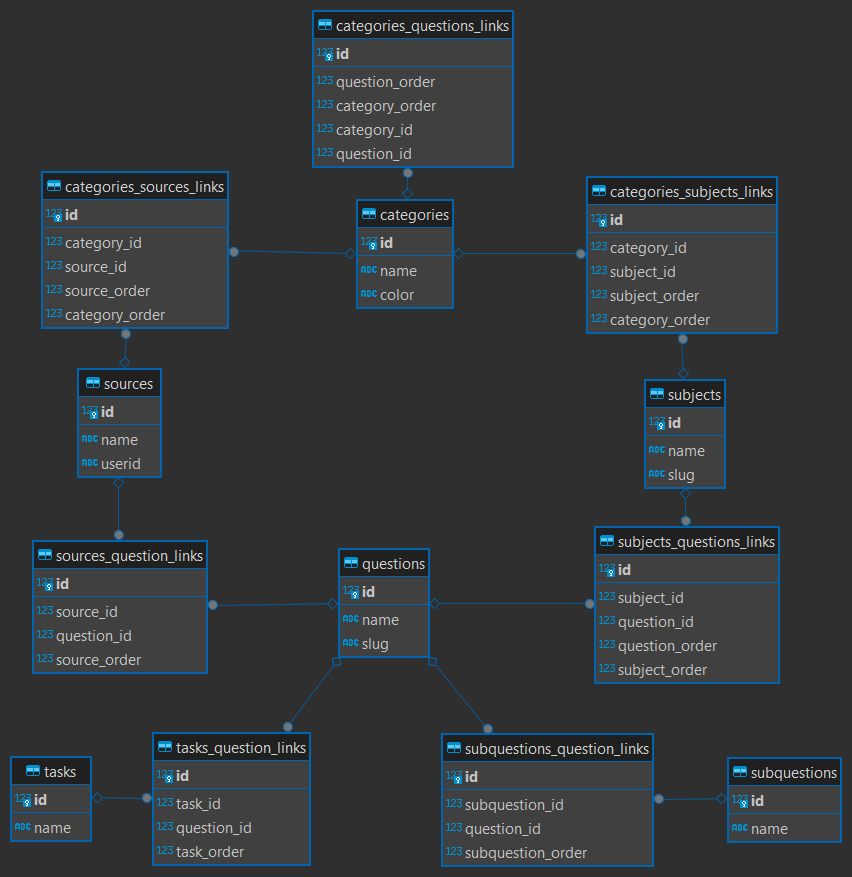
\includegraphics[width=0.7\linewidth]{image/scheme.png} 
	\caption{Ukázka databázového modelu}
\end{figure}

\section{Vercel}
Vercel je cloudová platforma pro nasazení a správu webových aplikací. Rozhodla jsem se využít tuto technologii, protože poskytuje jednoduchý způsob, jak nasadit statické a dynamické webové stránky, serverless funkcionalitu a další projekty spojené s vývojem webových a serverless aplikací.

\section{Autorizace}

\subsection{Clerk}
Clerk je autentizační platforma umožňující přihlašování pomocí hesel, poskytovatelů sociálních identit, jednorázových přístupových kódů e-mailem nebo SMS, vícefaktorového ověřování a základní správy uživatelů.

\subsubsection{Přidání ověřování a správy uživatelů do aplikace}
Clerk se nainstaloval pomocí příkazu 'npm install @clerk/nextjs'. Poté se v souboru '.env.local' vložil KEY kód. Aplikace se následně zabalila do <ClerkProvider>. 

\vspace{10pt}

\begin{lstlisting}[style=JavaScript, title={Kód}, caption={Ukázka <ClerkProvider> v layout.js}] 
	import { ClerkProvider } from "@clerk/nextjs";
	
	export default function RootLayout({ children }) {
		return (
			<ClerkProvider appearance={{ baseTheme: dark }}>
				<html lang="en">
					<body className={albert.className}>
						<ApolloWrapper>{children}</ApolloWrapper>
					</body>
				</html>
			</ClerkProvider>
		);
	}
\end{lstlisting}

\vspace{10pt}

Vyžadování ověřování pro přístup k aplikaci je řešeno v souboru 'middleware.ts'. Tímto způsobem je zabezpečena ochrana před neautorizovaným přístupem na tyto cesty, přičemž uživatelé, kteří nejsou ověřeni, budou přesměrováni na stránku pro přihlášení nebo na hlavní stránku.

\vspace{10pt}

\begin{lstlisting}[style=JavaScript, title={Kód}, caption={Ukázka kódu v middleware.ts}] 
	import { authMiddleware, redirectToSignIn } from "@clerk/nextjs";
	
	export const config = {
		matcher: ["/((?!.+\\.[\\w]+$|_next).*)", "/", "/(api|trpc)(.*)"],
	};
\end{lstlisting}

\newpage
Posledním krokem bylo vložit tlačítko <UserButton/>. Zde je <UserButton/> použit tak, že když je uživatel přihlášen, zobrazí se mu <UserButton/> a v opačném případě kdy je uživatel odhlášen, zobrazí se mu <SignInButton/>

\vspace{10pt}

\begin{lstlisting}[style=JavaScript, title={Kód}, caption={Ukázka kódu v middleware.ts}] 
	<button>
	<SignedIn>
		<UserButton />
	</SignedIn>
	<SignedOut>
	<SignInButton />
		</SignedOut>
	</button>
\end{lstlisting}

\subsection{Základní operace s uživatelským účtem}
Clerk poskytuje řadu základních operací s uživatelským účtem, které umožňují správu uživatelských účtů v aplikaci. Mezi tyto základní operace patří: 

\begin{itemize}
	\item Registrace
	\item Přihlášení
	\item Odhlášení
	\item Obnova hesla
	\item Správa účtů
	\item Ověření emailu
\end{itemize}

\newpage
\begin{figure}[h]
	\centering
	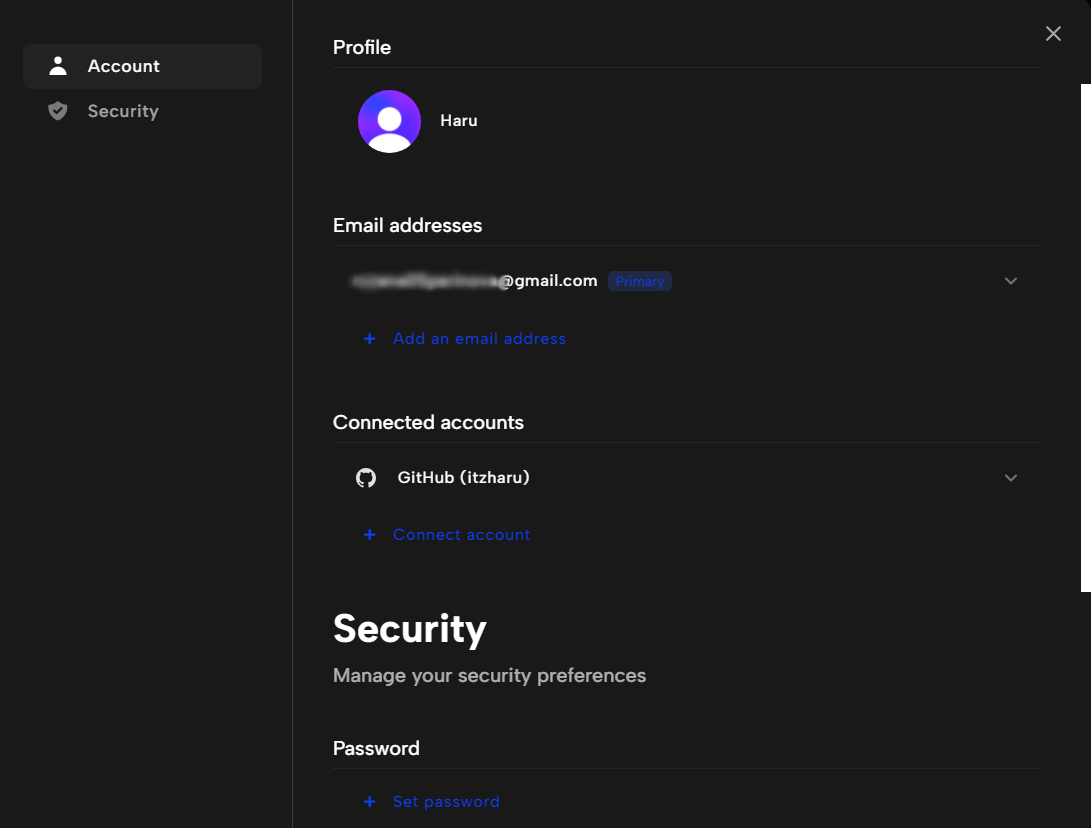
\includegraphics[width=0.8\linewidth]{image/clerk-profile.png} 
	\caption{Ukázka správy účtu}
\end{figure}

Clerk má předem vestavěnou správu účtů a nabízí řadu stylů, které se mohou aplikovat. V aplikaci bylo použito tmavé téma.

\vspace{10pt}

\begin{lstlisting}[style=JavaScript, title={Kód}, caption={Ukázka Clerk dark theme v layout.js}] 
	import { dark } from "@clerk/themes";
	
	export default function RootLayout({ children }) {
		return (
		<ClerkProvider appearance={{ baseTheme: dark }}>
			<html lang="en">
				<body className={albert.className}>
					<ApolloWrapper>{children}</ApolloWrapper>
				</body>
			</html>
		</ClerkProvider>
		);
	}
\end{lstlisting}

\chapter{Frontend}
\label{sec:frontend}

\section{React}
React je knihovna pro webová a nativní uživatelská rozhraní. Uživatelská rozhraní se skládají z jednotlivých částí nazývanými komponenty, které jsou napsané v jazyce JavaScript. React umožňuje snadno vytvářet interaktivní uživatelská rozhraní.

\subsection{React JSX}
JSX je zkratka pro JavaScript XML a umožňuje zapisovat prvky HTML v jazyce JavaScript a umisťovat je do DOM (Document Object Model) bez metod createElement() a/nebo appendChild().

\vspace{10pt}

\begin{lstlisting}[style=JavaScript, title={Kód}, caption={Ukázka využití JSX v page.js}] 
	return (
		<div>
			{data.subjects.data.map((subject) => {
				return (
					<div key={subject.slug}>
						<h3>
							{subject.attributes.Name}
						</h3>
					</div>
				);
			})}
		</div>
	);
\end{lstlisting}

\newpage
\subsection{React komponent}
Komponenty jsou nezávislé a opakovaně použitelné části kódu. Slouží ke stejnému účelu jako funkce JavaScriptu, ale pracují samostatně a vracejí HTML. Komponenty existují ve dvou typech, komponenty třídy a komponenty funkce. V aplikaci byl využit komponent funkce.

\subsection{React stav}
React komponenty mají vestavěný stavový objekt. Do objektu stavu se ukládají hodnoty vlastností, které patří komponentě. Když se stavový objekt změní, komponenta se znovu vykreslí.

\vspace{10pt}

\begin{lstlisting}[style=JavaScript, title={Kód}, caption={Ukázka useState() v Collapsible.jsx}] 
	import { useState } from "react";
	
	const [isOpened, setIsOpened] = useState(true);
	
	function toggleCollapsible() {
		setIsOpened((old) => !old);
	}>
\end{lstlisting}

\section{Tailwind CSS}
Tailwind CSS je populární CSS framework, který poskytuje sadu předdefinovaných utilit a tříd pro stylování webových stránek a aplikací. Díky Tailwind CSS se nemusí vytvářet vlastní CSS styl a rovnou do elementů se píší styly pomocí 'className'. Vybrala jsem si Tailwind CSS jako svůj framework, protože místo předdefinovaných komponentů či stylů umožňuje pracovat přímo s jednotlivými vlastnostmi stylu a díky tomu jsem si mohla stránku nastylovat přesně podle sebe.

\vspace{10pt}

\begin{lstlisting}[style=JavaScript, title={Kód}, caption={Ukázka useState() v Collapsible.jsx}] 
	<div
		className="relative py-1 px-2 w-fit h-full text-white rounded-l-sm"
		style={{ backgroundColor: tag.Color }}
	>
		{tag.Name}
	</div>
\end{lstlisting}

\newpage
\section{Apollo Client}
Apollo Client je komplexní knihovna pro správu stavu v jazyce JavaScript, která umožňuje spravovat místní i vzdálená data pomocí jazyka GraphQL. Pro propojení frontendu s backendem jsem se rozhodla využít Apollo Client pro jeho popularitu a taky protože většina tutoriálu na propojení Strapi GraphQL s React Next.js nabízela Apollo Client.

\subsection{Propojení frontendu s backendem}
Začala jsem instalací závislotí 'npm install @apollo/client graphql'. V souboru client.js jsem inicializovala Apollo Client pomocí uvedeného kódu.

\vspace{10pt}

\begin{lstlisting}[style=JavaScript, title={Kód}, caption={Ukázka inicializace Apollo Clientu v client.js}] 
import createUploadLink from "apollo-upload-client/createUploadLink.mjs";
import {
	NextSSRInMemoryCache,
	NextSSRApolloClient,
} from "@apollo/experimental-nextjs-app-support/ssr";
import { registerApolloClient } from
 "@apollo/experimental-nextjs-app-support/rsc";

let apolloClient;

export const { getClient } = registerApolloClient(() => {
	const client = new NextSSRApolloClient({
		cache: new NextSSRInMemoryCache(),
		link: createUploadLink({
			uri: "https://renowned-gift-126140aec8.strapiapp.com/graphql",
		}),
	});
	
	apolloClient = client;
	return client;
});

\end{lstlisting}

\newpage
Posledním krokem bylo obalit aplikaci wrapperem <ApolloProvider>.

\vspace{10pt}

\begin{lstlisting}[style=JavaScript, title={Kód}, caption={Ukázka komponentu <ApolloProvider> v client.js}] 
	<html lang="en">
		<body className={albert.className}>
			<ApolloWrapper>{children}</ApolloWrapper>
		</body>
	</html>
\end{lstlisting}

\chapter{Headless CMS}
\label{sec:headlessCMS}
Pro vývoj své webové aplikace jsem se rozhodla využít Headless CMS, protože je to jednoduchý způsob jak ukládat a spravovat své data na backendu, a to bez nutnosti vytváření vlastního backendu se serverem. Headless CMS umožňuje oddělit správu obsahu (backend) od prezentace obsahu (frontend), což přináší flexibilitu ve výběru frontendových technologií a zjednodušuje celkový vývoj aplikace.

\section{Strapi}
Původně jsem zvažovala možnost využití Hygraph, [] ale po následné konzultaci s panem učitelem jsme došli k závěru využití Strapi a později dockerizování aplikace.

\section{Strapi GraphQL}
GraphQL API umožňuje provádět dotazy a mutace pro interakci s typy obsahu prostřednictvím GraphQL pluginu v Strapi. Výsledky lze filtrovat, třídit a stránkovat. Ve své aplikaci jsem využila filtraci a třízení. Plugin měl také k dispozici playground, který jsem hodně využívala na dotazy předtím než jsem je aplikovala v kódu.

\vspace{10pt}

\begin{lstlisting}[style=JavaScript, title={Kód}, caption={Ukázka mutace v Content.js}] 
 	const uploadFile = gql`
	 	mutation ($file: Upload!) {
	 		upload(file: $file) {
	 			data {
	 				id
	 			}
	 		}
	 	}
	`;
\end{lstlisting}

\section{Strapi Cloud}

\chapter{Funkce aplikace}

\section{Nahrávání souboru}

\section{Mazání souboru}

\chapter*{Závěr}
	
	Závěr
	\renewcommand{\bibname}{Seznam použitých zdrojů}
	%% literatura
	\begin{thebibliography}{99}
		\bibitem{Next.js}Next.js by Vercel - The React Framework [Online]. [cit. 2023-01-12]. Dostupné z: \url{https://nextjs.org}
		\bibitem{GraphQL}GraphQL | A query language for your API [Online]. [cit. 2023-01-12]. Dostupné z: \url{https://graphql.org}
		\bibitem{Clerk}Clerk | Authentication and User Management [Online]. [cit. 2023-01-12]. Dostupné z: \url{https://clerk.com}
		\bibitem{W3Schools}W3schools Online Web Tutorials [Online]. [cit. 2023-01-13]. Dostupné z: \url{https://www.w3schools.com}
		\bibitem{Tailwind CSS}Tailwind CSS - Rapidly build modern websites without ever ... [Online]. [cit. 2023-01-13]. Dostupné z: \url{https://tailwindcss.com}
		\bibitem{Vercel}Vercel: Build and deploy the best Web experiences with The ... [Online]. [cit. 2023-01-13]. Dostupné z: \url{https://vercel.com}
		\bibitem{Apollo Client}Introduction to Apollo Client [Online]. [cit. 2023-01-14]. Dostupné z: \url{https://www.apollographql.com/docs/react/}
		\bibitem{RCS}React Server Components in Next.js 13 [Online]. [cit. 2023-01-14]. Dostupné z: \url{https://blog.logrocket.com/react-server-components-next-js-13/}
		\bibitem{Strappi}Strapi - Open source Node.js Headless CMS
		 [Online]. [cit. 2023-01-14]. Dostupné z: \url{https://strapi.io}
	\end{thebibliography}
	
	%% obrázky 
	\listoffigures
	
	\appendix %% začínají přílohy
	
	\titleformat{\chapter}[block]{\scshape\bfseries\LARGE}{Příloha \thechapter}{10pt}{\vspace{0pt}}[\vspace{-22pt}] %% nastavení nadpisu u příloh
	
	
\end{document}